\chapter{Aspectos conceituais}
\label{CAP2}

A seguir serão explicados os conceitos fundamentais que possibilitam a execução deste trabalho. 

% apresentar conceitos empregados e revisao da literatura (parte toerica do trab)

\section{O padrão OBD-II}

Criado na década de 1990 para gerar controle sobre as emissões de gás carbônico dos carros\textsuperscript{[5]}, hoje define um protocolo padronizado para comunicar parâmetros internos do veículo. O padrão OBD-II foi uma extensão do padrão OBD-I, uniformizando esse tipo de conector em casos em geral, começando a ser adotado no Brasil a partir de 2010\textsuperscript{[4]}.

A comunicação é feita através de uma conexão física que normalmente pode ser encontrada abaixo do volante do motorista\textsuperscript{[5]}, conforme indicado pela figura \ref{fig:obd2_conn}. Nesse padrão de conexão e comunicação, é definida uma interface por onde parâmetros internos de um veículo podem ser monitorados.

As mensagens definidas pelo OBD-II têm cada uma um PID (\textit{Parameter ID}). O conjunto comum de PIDs de serviços que podem ser solicitados pela porta OBD-II e para que servem pode ser visto na tabela \ref{Tb:tab1}\textsuperscript{[3]}.

\begin{table}[]
% \begin{adjustbox}{width=\textwidth}
\begin{tabular}{cc}
\rowcolor[HTML]{656565} 
{\color[HTML]{FFFFFF} Service / Mode (hex)} & {\color[HTML]{FFFFFF} Description}                                                                    \\
01                                          & Show current data - I/M Monitors and Live Data                                                        \\
02                                          & Show Freeze Frame (FF) Data                                                                           \\
03                                          & Show Stored Diagnostic Trouble Codes                                                                  \\
04                                          & Clear/Erase Diagnostic Trouble Codes and stored values                                                \\
05                                          & Test results, oxygen sensor monitoring (non CAN only)                                                 \\
06                                           & Test results, other component/system monitoring (Test results, oxygen sensor monitoring for CAN only) \\
07                                           & Show pending Diagnostic Trouble Codes (detected during current or last driving cycle)                 \\
08                                           & Control operation of on-board component/system (EVAP)                                                 \\
09                                          & Request Vehicle Information (VIN)                                                                     \\
0A                                          & Permanent Diagnostic Trouble Codes (DTCs) (Cleared DTCs)                                             
\end{tabular}
\end{table}


É importante notar que os serviços do padrão OBD-II comuns a todos os carros sempre começam com o dígito zero (hexadecimal), por isso, serviços específicos de cada fabricante precisam começam a partir do código 0x10.

\begin{figure}[hp]
    \centering
    
    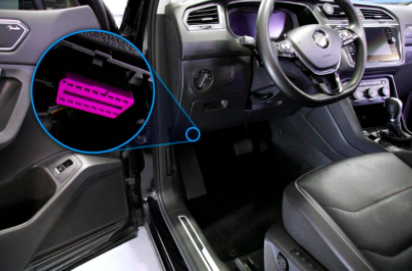
\includegraphics[]{figures/localizacao_obd2.png}
    
    \caption{Posição da porta OBD-II em um carro\textsuperscript{[5]}}
    
    \label{fig:obd2_conn}
\end{figure}

Os dados, que podem ser coletados de qualquer carro, são explicitados na tabela \ref{Tb:tab2}\textsuperscript{[3]}.





Embora não esteja explicitamente representado na tabela, os PIDs 0x00, 0x20, 0x40, etc., ou seja, a cada 32 valores de PID, possuem um parâmetro dedicado exclusivamente para indicar quais, dentre os PIDs subsequentes, são fornecidos pelo veículo em questão. Esses PIDs de marcação, por assim dizer, utilizam 4 \textit{bytes} para comunicar quais dos próximos PIDs estão disponíveis, utilizando cada \textit{bit} como uma \textit{flag} binária. 

Na figura \ref{fig:bitwise_obd2} é possível visualizar como esse processo é feito, usando como exemplo o valor \textit{0xBE1FA813} para representar os 4 \textit{bytes} oferecidos\textsuperscript{[3]}.

\begin{figure}[hp]
    \centering
    
    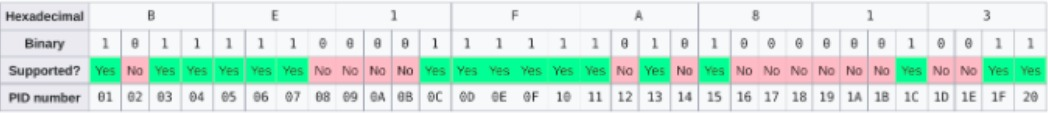
\includegraphics[scale=0.42]{figures/tabela_dados_disponiveis.jpeg}
    
    \caption{Divisão bit a bit da mensagem OBD-II informando os serviços disponíveis\textsuperscript{[3]}}
    
    \label{fig:bitwise_obd2}
\end{figure}


A coleta de fato dos dados relevantes é feita por uma aplicação desenvolvida \textit{a priori} ao começo do projeto, a qual já era capaz de comunicar-se corretamente com a interface OBD\textsuperscript{[43]}.

Essa aplicação acelerou a criação da infraestrutura proposta por este trabalho, uma vez que adiantou o primeiro passo da estratégia \textit{bottom-up} que permeou o projeto.

% Please add the following required packages to your document preamble:
% \usepackage[table,xcdraw]{xcolor}
% If you use beamer only pass "xcolor=table" option, i.e. \documentclass[xcolor=table]{beamer}
\begin{table}[]
\begin{tabular}{ccccccc}
\rowcolor[HTML]{C0C0C0} 
{\color[HTML]{FFFFFF} \textbf{PIDs(hex)}} & {\color[HTML]{FFFFFF} \textbf{PID(Dec)}} & {\color[HTML]{FFFFFF} \textbf{Data bytes returned}} & {\color[HTML]{FFFFFF} \textbf{Description}} & {\color[HTML]{FFFFFF} \textbf{Min value}} & {\color[HTML]{FFFFFF} \textbf{Max value}} & {\color[HTML]{FFFFFF} \textbf{Units}} \\
04                                         & 4                                        & 1                                                   & Calculated engine load                      & 0                                         & 100                                       & \%                                    \\
0C                                        & 12                                       & 2                                                   & Engine speed                                & 0                                         & 16,383.75                                 & rpm                                   \\
0D                                        & 13                                       & 1                                                   & Vehicle speed                               & 0                                         & 255                                       & km/h                                  \\
0F                                        & 15                                       & 1                                                   & Intake air temperature                      & -40                                       & 215                                       & °C                                    \\
1F                                        & 31                                       & 2                                                   & Run time since engine start                 & 0                                         & 65,535                                    & seconds                               \\
33                                        & 51                                       & 1                                                   & Absolute Barometric Pressure                & 0                                         & 255                                       & kPa                                   \\
46                                        & 70                                       & 1                                                   & Ambient air temperature                     & -40                                       & 215                                       & °C                                    \\
47                                        & 71                                       & 1                                                   & Absolute throttle position B                & 0                                         & 100                                       & \%                                    \\
49                                        & 73                                       & 1                                                   & Accelerator pedal position D                & 0                                         & 100                                       & \%                                    \\
51                                        & 81                                       & 1                                                   & Fuel Type                                   & -                                         & -                                         & -                                     \\
52                                        & 82                                       & 1                                                   & Ethanol fuel \%                             & 0                                         & 100                                       & \%                                    \\
5A                                        & 90                                       & 1                                                   & Relative accelerator pedal position         & 0                                         & 100                                       & \%                                    \\
5B                                        & 91                                       & 1                                                   & Hybrid battery pack remaining life          & 0                                         & 100                                       & \%                                    \\
5C                                        & 92                                       & 1                                                   & Engine oil temperature                      & -40                                       & 210                                       & °C                                    \\
5D                                        & 93                                       & 2                                                   & Fuel injection timing                       & -210.00                                   & 301992                                    & °                                     \\
5E                                        & 94                                       & 2                                                   & Engine fuel rate                            & 0                                         & 3212.75                                   & L/h                                   \\
61                                        & 97                                       & 1                                                   & Driver's demand engine - percent torque     & -125                                      & 130                                       & \%                                    \\
62                                        & 98                                       & 1                                                   & Actual engine - percent torque              & -125                                      & 130                                       & \%                                    \\
63                                        & 99                                       & 2                                                   & Engine reference torque                     & 0                                         & 65,535                                    & Nm                                    \\
64                                        & 100                                      & 5                                                   & Engine percent torque data                  & -125                                      & 130                                       & \%                                    \\
70                                        & 112                                      & 10                                                  & Boost pressure control                      & -                                         & -                                         & -                                     \\
83                                        & 131                                      & 9                                                   & NOx sensor                                  & -                                         & -                                         & -                                     \\
8E                                        & 142                                      & 1                                                   & Engine Friction - Percent Torque            & -125                                      & 130                                       & \%                                   
\end{tabular}
\end{table}

\subsection{Trabalhos relacionados-OBD-II}

O estudo de \cite{Ahmadi-Assalemi, 2021} envolveu uma rota com diversas condições, como rotatórias, semáforos e ruas com zonas de alta e baixa velocidade.  O veículo utilizado estava equipado com Sistema de Posicionamento Global (GPS) e porta de Diagnóstico a Bordo (OBD2), padrão para carros fabricados a partir de 2012.  Diferenças nos padrões de direção foram encontradas para distinguir entre motoristas do sexo feminino e masculino com base em variações na aceleração longitudinal, especialmente na velocidade de direção, torque e espectro de RPM.
O processo de como foram coletados os dados neste trabalho pode ser visto na figura \ref{fig:obd2_profiling}.

O trabalho de \cite{Navneeth,2020} aborda a importância do perfil do motorista na garantia da segurança. Ele fornece uma visão geral da base de conhecimento para o consumidor sobre Diagnóstico a Bordo (OBD) e Perfil do Motorista. O OBD auxilia na manutenção do carro, identificando códigos de problemas do controle do motor por meio de um aplicativo Android. 

Quanto ao perfil do comportamento do motorista, o artigo propõe duas abordagens: uma simples e imediata, utilizando coordenadas GPS no mesmo aplicativo Android proposto para diagnósticos a bordo, e outra mais detalhada e inovadora, baseada em parâmetros do motor do carro e utilizando técnicas de análise de dados e aprendizado de máquina não supervisionado.
Na figura \ref{fig:tabela_score} é possível ver a classificação utilizado pelo autor.

O artigo de \cite{Malik Meenakshi, 2023} aborda métodos de análise detalhada do comportamento do motorista(Driver Behaviour). A análise dos dados é fundamental para prever a atenção, distração e fadiga do motorista em relação ao ambiente e ao veículo. Muitos acidentes resultam de comportamentos de condução arriscados, destacando a necessidade de identificar e abordar esses comportamentos para combater o aumento de acidentes de trânsito. O trabalho explora informações do sistema de diagnóstico veicular "OBD-II"  e algoritmos de aprendizado de máquina (ML).

A condução agressiva é caracterizada por variações abruptas na aceleração (aumento de velocidade) ou desaceleração (freagem). Sensores, acelerômetros e giroscópios são empregados para medir essas mudanças. Os valores de aceleração ou desaceleração também podem ser determinados pela variação na velocidade de um GPS instalado no veículo. Assim como no caso da velocidade, acelerações ou desacelerações responsáveis ou arriscadas definem o comportamento do motorista \cite{Malik Meenakshi, 2023}.

O RPM(rotações por minuto) indica a carga de trabalho do motor.  Os fabricantes de veículos recomendam RPMs ideais para otimizar a eficiência do combustível. Seguir essas recomendações em relação à velocidade, troca de marchas e RPMs resulta na melhor economia de combustível. Portanto, a análise do comportamento do motorista revela que variações nas RPM, fora das recomendações do fabricante, estão associadas a um aumento no consumo de combustível \cite{Malik Meenakshi, 2023}.




\begin{figure}[hp]
    \centering
    
    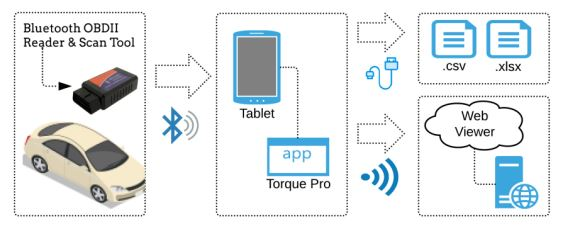
\includegraphics[]{figures/obd2_profiling.jpg}
    
    \caption{Processo de coleta de dados\textsuperscript{[44]}.}
    
    \label{fig:obd2_profiling}
\end{figure}

\begin{figure}[hp]
    \centering
    
    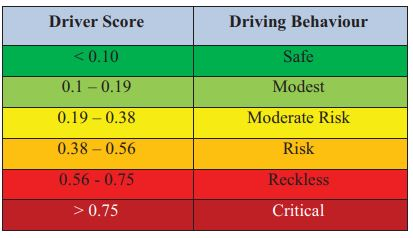
\includegraphics[]{figures/tabela_score.jpg}
    
    \caption{Tabela de Score\textsuperscript{[45]}.}
    
    \label{fig:tabela_score}
\end{figure}

\section{O Padrão vehicle-to-everything(V2X)}

A tecnologia sem fio veicular moderna possibilita que os veículos troquem informações a qualquer momento, de qualquer lugar, para qualquer rede, formando as plataformas de comunicação vehicle-to-everything(V2X). Apesar dos benefícios, as aplicações V2X também enfrentam grandes desafios de segurança e privacidade. \cite{M. Hasan, 2020}.

Na figura \ref{fig:nos_de_comunicacao}, ilustra-se uma infraestrutura de chave pública (PKI) em alto nível para comunicações V2X. O nó de comunicação (por exemplo, veículo) é uma entidade final do sistema que solicita certificados da PKI e se comunica com outras entidades finais. A Autoridade Certificadora Raiz (RCA) é a raiz de confiança para todos os certificados. Ela fornece certificados às entidades de autorização para emitir certificados aos nós de comunicação. O centro de distribuição fornece informações de confiança atualizadas necessárias para validar informações recebidas de uma autoridade PKI legítima e autorizada. O operador registra nós de comunicação e atualiza as informações necessárias nas entidades de autorização \cite{M. Hasan, 2020}.

\begin{figure}[hp]
    \centering
    
    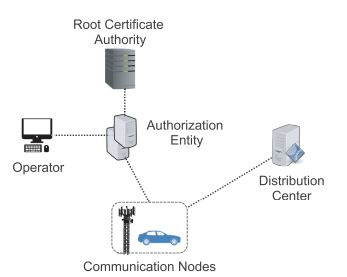
\includegraphics[]{figures/nos_de_comunicacao.jpg}
    
    \caption{Nós de comunicação\textsuperscript{[47]}.}
    
    \label{fig:nos_de_comunicacao}
\end{figure}

O artigo de \cite{Xuyu Wang, 2017} categoriza as aplicações V2X em duas grandes classes: (i) aplicações de segurança V2X e (ii) aplicações não relacionadas à segurança V2X. A figura \ref{fig:v2x_seguranca} mostra as aplicações de segurança. Com o uso da tecnologia V2X é possível detectar colisões, a presença de pedestres e casos de veículos em emergências.

Já as aplicações V2X não relacionadas à segurança concentram-se principalmente em eficiência e gerenciamento de tráfego, visando melhorar o fluxo de veículos, coordenação de tráfego e assistência.






\begin{figure}[hp]
    \centering
    
    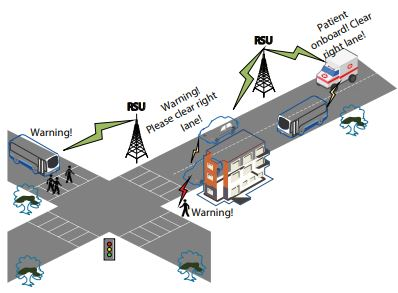
\includegraphics[]{figures/v2x_seguranca.jpg}
    
    \caption{Aplicações de segurança\textsuperscript{[48]}.}
    
    \label{fig:v2x_seguranca}
\end{figure}


\section{Transmissão de dados}

A implementação do \textit{Bluetooth} neste projeto proporciona uma solução eficaz para a comunicação entre a porta OBD do veículo e o \textit{smartphone} do motorista. 

% Essa escolha oferece uma conectividade sem fio e em tempo real com o aplicativo, simplificando a transmissão de dados.

A abordagem \textit{wireless} elimina a necessidade de cabos físicos, contribuindo para uma integração mais simplificada do sistema. A eficiência energética do \textit{Bluetooth} assegura uma transmissão de dados sem fio sem prejudicar significativamente o consumo de bateria do aparelho celular.

% Além disso, a transmissão \textit{Bluetooth} facilita a interação direta entre o sistema de geração de dados e os usuários, possibilitando a visualização em tempo real de informações de condução. Essa integração sem fio não apenas aprimora a experiência do usuário, mas também amplia as possibilidades de interatividade e controle, tornando o sistema mais acessível e fácil de usar.


 \begin{figure}[hp]
    \centering
    
    
\includegraphics[scale=0.4]{figures/bluetooth.png}
    
    \caption{Logo do Bluetooth.}
    
\end{figure}

\section{Armazenamento em nuvem}
O Amazon Web Services\textsuperscript{[10]} (AWS) foi o serviço de nuvem escolhido para o armazenamento dos dados do projeto, destacando-se por suas vantagens em segurança, escalabilidade e praticidade. 

A AWS oferece uma infraestrutura robusta com elevados padrões de segurança, garantindo a proteção avançada dos dados, enquanto sua escalabilidade permite uma adaptação eficiente às crescentes demandas do projeto, mantendo a eficiência operacional. Essa escolha proporciona um ambiente de nuvem que atende às exigências do projeto e estabelece uma base sólida para o desenvolvimento futuro.

A base de dados escolhida usa MySQL e foi hospedada em uma instância RDS. Todas as informações coletadas através do aplicativo desenvolvido foram armazenadas nesse serviço.

% Informações, como localização, velocidade e aceleração, podem então ser usadas para geração de gráficos e métricas essenciais na avaliação do perfil do motorista.

A combinação do Amazon RDS com a base de dados MySQL oferece uma solução eficiente e escalável para o armazenamento de dados, atendendo às necessidades do projeto e garantindo alta disponibilidade e segurança dos dados.




% \begin{table}[]
% \begin{tabular}{lllll}
% \multicolumn{5}{c}{\textbf{resumo da estimativa}}                                       \\
%                        &  &                       &  &                                  \\
% \textbf{custo inicial} &  & \textbf{custo Mensal} &  & \textbf{Custo total em 12 meses} \\
%                        &  &                       &  &                                  \\
% 0.00 USD               &  & 14.71 USD             &  & 176.52 USD                       \\
%                        &  &                       &  &                                 
% \end{tabular}
% \end{table}


\begin{table}[]

    \caption{Custo projetado da instância da AWS.}
    \label{Tb:tab_escolhas_instancia}
    \centering
    
    % \begin{tabular}{lllll}
    \begin{adjustbox}{width=\textwidth}
        \begin{tabular}{ccc p{6cm} ccc}
            \rowcolor[HTML]{C0C0C0} 

            \hline
            
            \multicolumn{1}{|l|}{\textbf{Custo inicial}}  & \multicolumn{1}{|l|}{\textbf{Custo Mensal}}  & \multicolumn{1}{|l|}{\textbf{Custo Total em 12 Meses}} \\

            \hline
            
            \multicolumn{1}{|l|}{0,00 USD}  & \multicolumn{1}{|l|}{14,71 USD}    & \multicolumn{1}{|l|}{176,52 USD}  \\

            \hline
        \end{tabular}
    \end{adjustbox}
\end{table}


            % \multicolumn{5}{c}{\textbf{resumo da estimativa}}                                       \\
                                   % &  &                       &  &                                  \\

% A região do Leste da Virgina é conhecida por ter uma alta densidade de \textit{data centers}. Isso resulta em eficiência operacional e redução de custos.

A instância escolhida para o RDS foi a \textbf{db.t3.micro}, pois ela é uma unidade de processamento adequada para cargas de trabalho leves e é comumente usada para ambientes de desenvolvimento, testes ou pequenas aplicações que não exigem muitos recursos.

Foi cogitado fazer uso de um RDS Proxy, que é um serviço que facilita a escalabilidade e a alta disponibilidade para as conexões de banco de dados, mas como este projeto trata-se de um protótipo, não houve preocupações quanto a grandes cargas de trabalho e essa decisão foi descartada. 

% Logo, essa opção não foi escolhida. 

% Ele ajuda a melhorar o desempenho e a segurança ao gerenciar as conexões entre seus aplicativos e instâncias de banco de dados RDS. 

% Isso é especialmente útil em ambientes onde há flutuações na carga de trabalho. 

Também não há necessidade de haver um ambiente de zona de disponibilidade múltipla para garantir escalabilidade, pois haveria custo adicional para o MVP. Por isso, a instância RDS foi configurada para o modo Single-AZ. E a capacidade de armazenamento foi limitada a 20 GiB.


% \begin{table}[]
% \begin{tabular}{|ll|}
% \hline
% \multicolumn{1}{|l|}{\textbf{Região}}                 & Virgínia     \\ \hline
% \multicolumn{1}{|l|}{}                                &              \\ \hline
% \multicolumn{2}{|c|}{\textbf{Especificação das instancias do MySQL}} \\ \hline
% \multicolumn{1}{|l|}{Quantidade de Instancias MYSQL}  & 1            \\ \hline
% \multicolumn{1}{|l|}{tipo da instancia}               & db.t3.micro  \\ \hline
% \multicolumn{1}{|l|}{vCPU}                            & 2            \\ \hline
% \multicolumn{1}{|l|}{Memória}                         & 1GiB         \\ \hline
% \end{tabular}
% \end{table}




\begin{table}[h]

    \caption{Parâmetros de escolha da instância da AWS.}
    \label{Tb:tab_escolhas_instancia}
    \centering
    
    \begin{adjustbox}{width=\textwidth}
        \begin{tabular}{ccc p{6cm} ccc}
            \rowcolor[HTML]{C0C0C0} 
        
        % \begin{tabular}{|ll|}
            \hline
            
            \multicolumn{2}{|c|}{\textbf{Especificação das instâncias do MySQL}} \\ 
            
            \hline
            
            \multicolumn{1}{|l|}{Região}                          & \multicolumn{1}{|l|}{ US East(N.Virginia)}     \\ 
            
            \hline
            
            \multicolumn{1}{|l|}{Quantidade de instâncias MySQL}  & \multicolumn{1}{|l|}{1}            \\ 
            
            \hline
            
            \multicolumn{1}{|l|}{Tipo da instância}               & \multicolumn{1}{|l|}{db.t3.micro}  \\ 
            
            \hline
            
            \multicolumn{1}{|l|}{vCPU}                            & \multicolumn{1}{|l|}{2}           \\ 
            
            \hline
            
            \multicolumn{1}{|l|}{Memória}                         & \multicolumn{1}{|l|}{1GiB}         \\ 
            
            \hline
    
        \end{tabular}
    \end{adjustbox}
\end{table}

% \begin{table}[h]

%     \caption{Parâmetros de escolha da instância da AWS - aaa.}
%     \label{Tb:tab_escolhas_instancia}
%     \centering
    
%     \begin{adjustbox}{width=\textwidth}
%         \begin{tabular}{ccc p{6cm} ccc}
%     % \centering
        
%         % \begin{tabular}{|ll|}
%             \hline
%             \multicolumn{2}{|c|}{\textbf{Especificação das instâncias do MySQL}} \\ \hline
%             % \multicolumn{1}{|l|}{Região}                          & Virgínia     \\ \hline
%             % \multicolumn{1}{|l|}{Quantidade de instâncias MySQL}  & 1            \\ \hline
%             % \multicolumn{1}{|l|}{Tipo da instância}               & db.t3.micro  \\ \hline
%             \multicolumn{1}{|l|}{Região}  & \multicolumn{1}{l|}{Virgínia}    \\ \hline
%             \multicolumn{1}{|l|}{Quantidade de instâncias MySQL}  & \multicolumn{1}{l|}{1}    \\ \hline
%             \multicolumn{1}{|l|}{Tipo da instância}  & \multicolumn{1}{l|}{db.t3.micro}    \\ \hline
%             \multicolumn{1}{|l|}{vCPU}  & \multicolumn{1}{l|}{2}    \\ \hline
%             \multicolumn{1}{|l|}{Memória}  & \multicolumn{1}{l|}{1GiB}    \\ \hline
%             % \multicolumn{1}{|l|}{Memória}                         & 1GiB         \\ \hline
    
%         \end{tabular}
%     \end{adjustbox}
% \end{table}